%=========PROBLEM 2============================================
\section*{Problem 2}

The AzTEC mm-wavelength camera completed a large survey of the COSMOS field in search for sub-millimeter galaxies. 
A typical source detection is between 4 and 10 sigma level. 
Before analyzing the data, is important to understand the noise properties of the camera. 
To do this, noise maps are produced. A noise map is a map with little to no astronomical signal. 
In this problem, a noise map of AzTEC was given. We need to produce two histograms, one linear and another in semi-log form, of the data within the center 20 arc-minutes of the map. 
The pixel size is $3 \times 3$ arc-seconds.

The steps followed to do the histograms are the following:

\begin{enumerate}
    \item Import fits file and read header.
    
    FITS stands for Flexible Image Transport System. It is a standard used mainly in astronomy to save data of the observations in a standard way. To import a fits file into Python so that the data can be accessed, a viewer is needed. It was recommended to use PyFits which was ported to Astropy as "astropy.io.fits". For this reason, astropy was used for this and subsequent problems as needed. 
    
    Once the fits viewer was imported, 
    \lstinline[columns=fixed, style=Python]{fits.open()} 
    will open the fits file. The fits file is compose of a list of objects which are compose of two parts: a header and the data. The header is were the metadata of the image is located. It gives information such as the timestamp, the instrument used, the number of axes, the number of pixels, etc. These parameters can be put into a variable by calling them by their label. 
    
    \item Extract the data of the centered 20 arcminutes.
    
    A mask is used to achieve this step. A mask is a matrix of the same size as the data which contains boolean values. If True, the data will stay as is and if False, the data will be turn into zero. This process will only "make visible" the data we are interested. 
    
    The mask "shape" will be a circle since the information needed is the within 20 arcminutes of the center of the map. Using the header, the location of the central pixel can be estimated by taking the length of the axis and divide it by 2. It is known that the equation of the circle is given by 
    \begin{equation} \label{eq:circle}
        r = \sqrt{(x-x_0)^2 + (y-y_0)^2}
    \end{equation}
    where $x_0$ and $y_0$ are the coordinates of the center and $r$ is the radius of the circle. 
    
    The radius of the circle is 20 arcminutes which transformed into pixels, given that each pixel is 3 arcseconds, is 
    \begin{equation}\label{eq:radiusInPixels}
        r= 20' \times \frac{60''}{1'} \times \frac{1  \mathrm{pixel}}{3''} = 400 \mathrm{pixel}
    \end{equation}
    
    Comparing the right hand of equation \ref{eq:circle} bigger than r in pixels, outputs a boolean array with same dimensions as the data, in other words, it creates the mask. The mask is applied to the data and later trimmed so it will contain the information wanted. 
    
    \item Create histograms.
    
    An histogram shows how many times the values in a range are repeated. The range is given by the bin size. Since the values are being counted, the positions of the values are not important at this point. The \lstinline[columns=fixed, style=Python]{data.flatten()} command makes the 2 dimensional array into a 1 dimensional array. After this, the data is ready to get the histogram. 
    
    The histograms of the values are given by Figure \ref{fig:histograms}. 
    
    \begin{figure}[]
        \centering
        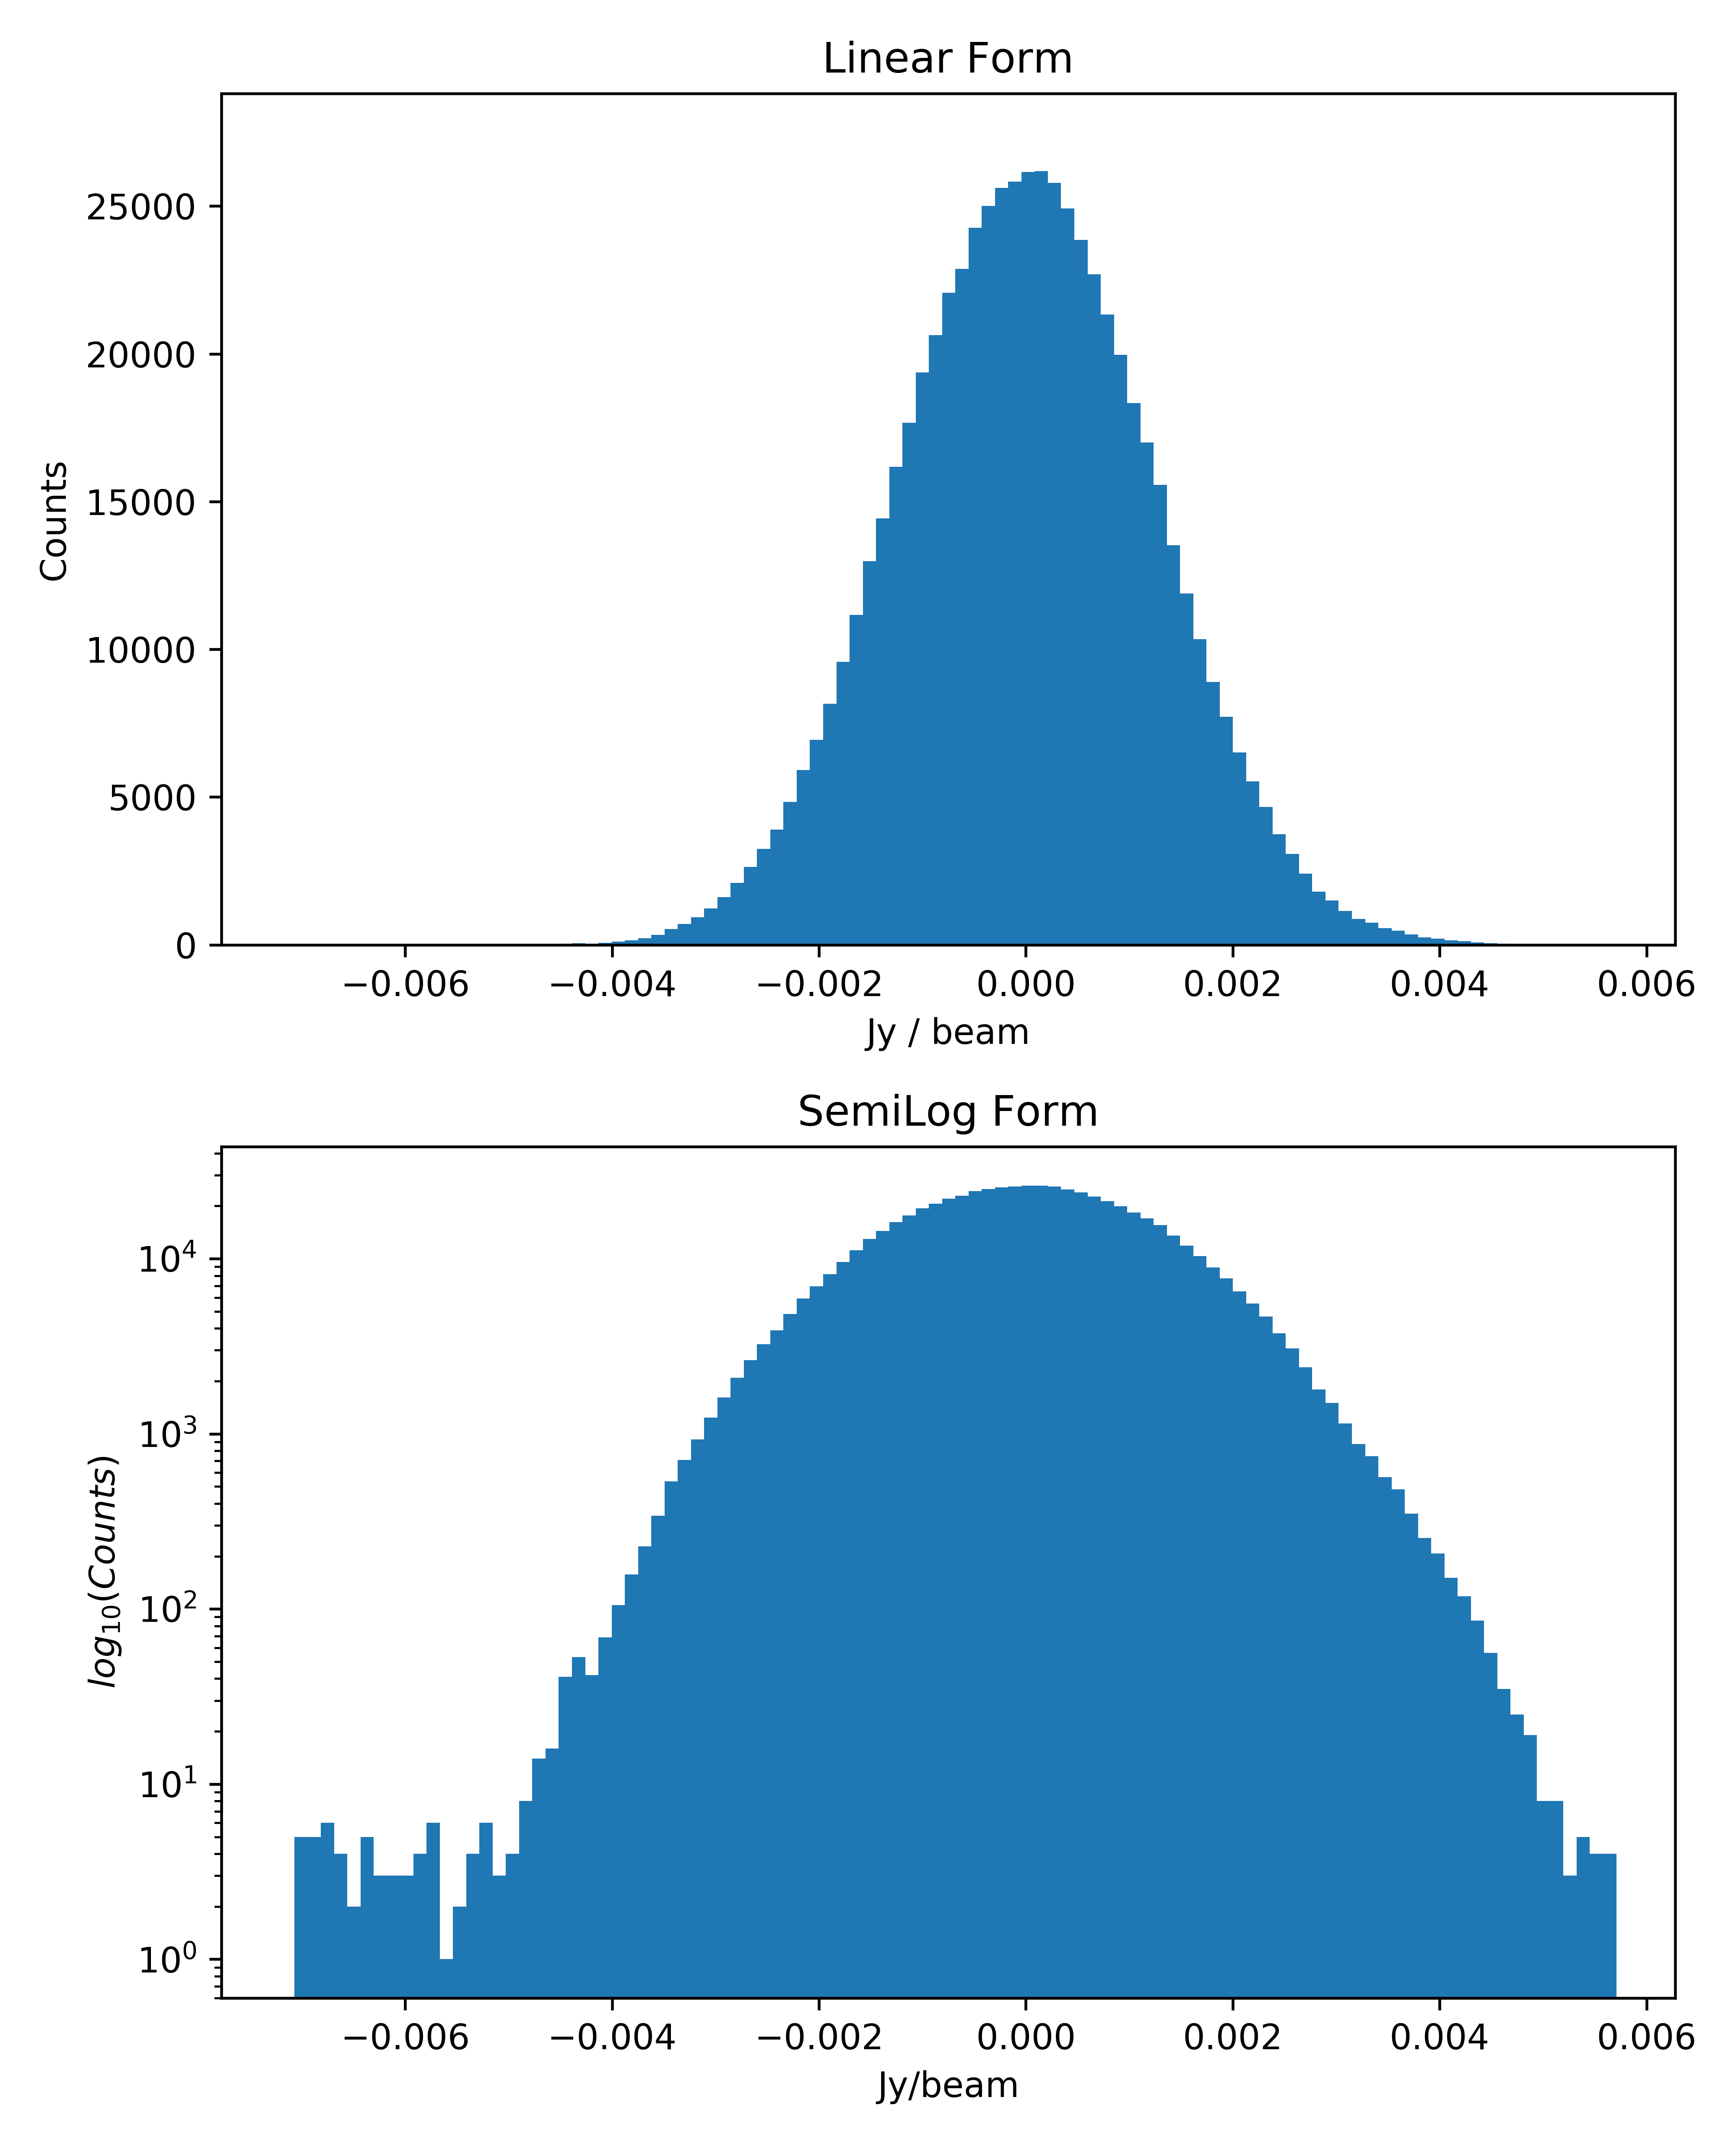
\includegraphics{figures/hw01prob1-2fig1.png}
        \caption{Histograms of the noise map of AzTEC. Top: Histogram in a linear form. Bottom: Histogram in a semi-log form.}
        \label{fig:histograms}
    \end{figure}
    
     \item \textbf{Customize the plot to achieve a readable and understandable plot.}
     
\end{enumerate}

The histogram in its linear form shows a bell-like shape. This shape is associated to a normal distribution or to a Gaussian. The mean of the data will be the center of this shape. This suggests that the noise is produced by a random process.

The histogram in its semilog form shows a more rounded shape.This shows that most values are near the center. 
